% Gets the style guide to apply to the document such as font sizes for various wrappers, spacing before and after sections, etc.
% \documentclass[letterpaper,twoside,openright]{document-formatting} %this is for double sided alternating the extra margin on left and right pages
\documentclass[letterpaper,onesided,openright]{document-formatting}
% NOTE THAT THE SECOND LAST LINE OF DOCUMENT-FORMATTING.CLS LETS YOU CHANGE THE CITATION STYLE

% Hides addition of external plugins
% This package is for charsets (default)
\usepackage[utf8]{inputenc}

% The principal package in the AMS-LATEX distribution. It adapts for use in LATEX most of the mathematical features found in AMS-TEX; it is highly recommended as an adjunct to serious mathematical typesetting in LATEX. (https://ctan.org/pkg/amsmath?lang=en)
\usepackage{amsmath}
\usepackage{mathdots}

% better absolute brackets
\usepackage{mathtools}
\DeclarePairedDelimiter\abs{\lvert}{\rvert}%
\DeclarePairedDelimiter\norm{\lVert}{\rVert}%

% Swap the definition of \abs* and \norm*, so that \abs
% and \norm resizes the size of the brackets, and the 
% starred version does not.
\makeatletter
\let\oldabs\abs
\def\abs{\@ifstar{\oldabs}{\oldabs*}}
%
\let\oldnorm\norm
\def\norm{\@ifstar{\oldnorm}{\oldnorm*}}
\makeatother

% Algorithm2e is an environment for writing algorithms. (https://ctan.org/pkg/algorithm2e?lang=en)
\usepackage{algorithm2e}

 % The package builds upon the graphics package, providing a key-value interface for optional arguments to the \includegraphics command. This interface provides facilities that go far beyond what the graphics package offers on its own. (https://ctan.org/pkg/graphicx?lang=en)
\usepackage{graphicx}

% This package is for font and sizing the captions on figures and tables.
\usepackage[labelfont=bf,font={footnotesize,singlespacing}]{caption}

% A LATEX2ε package to help change the style of any or all of LATEX's sectional headers in the article, book, or report classes. Examples include the addition of rules above or below a section title. (https://ctan.org/pkg/sectsty?lang=en)
\usepackage{sectsty}
% \subsectionfont{\small}

% The xr package is used for cross-referencing across multiple independent documents. For example, you would use the xr package if you had two separate files in a project, File1.tex and File2.tex, and you would like to have a reference in File1.tex to something labelled in File2.tex, without including File2.tex in File1.tex. (https://www.overleaf.com/learn/how-to/Cross_referencing_with_the_xr_package_in_Overleaf)
\usepackage{xr}

% The hyperref package is used to handle cross-referencing commands in LATEX to produce hypertext links in the document. (https://ctan.org/pkg/hyperref?lang=en)
\usepackage{hyperref}

% The package enhances LATEX’s cross-referencing features, allowing the format of references to be determined automatically according to the type of reference. (https://ctan.org/pkg/cleveref?lang=en)
\usepackage{cleveref}

% Package to show and highlight code
\usepackage{listings}

% Allow Multicolumn sections
\usepackage{blindtext} % for adding some random text data in sections
\usepackage{multicol} % for making multi column layouts

% Allow Drawing of decay schemes
\usepackage{tikz}
\usetikzlibrary{positioning}

% Allow the use of Chemstry notation
\usepackage{mhchem}

% To make sure that Latex doesn't reposition tables
\usepackage{float}
\floatstyle{plaintop}
\restylefloat{table}
% \restylefloat{figure}

\usepackage[section]{placeins}

% all figure file names relative to this path
%\graphicspath{ {../Figures/} } %NOT REALLY NEEDED IF YOU JUST DIRECT LINK INSTEAD OF RELATIONAL LINK

%allow right aligned columns
\usepackage{array,booktabs,ragged2e}
\newcolumntype{R}[1]{>{\RaggedLeft\arraybackslash}p{#1}}

%colour table rows
\usepackage{color, colortbl}
\definecolor{Gray}{gray}{0.9}

%%% HELPER CODE FOR DEALING WITH EXTERNAL REFERENCES
\makeatletter
\newcommand*{\addFileDependency}[1]{
  \typeout{(#1)}
  \@addtofilelist{#1}
  \IfFileExists{#1}{}{\typeout{No file #1.}}
}
\makeatother

\newcommand*{\myexternaldocument}[1]{
    \externaldocument{#1}
    \addFileDependency{#1.tex}
    \addFileDependency{#1.aux}
}

%%% END HELPER CODE

% Page numbering
\usepackage{fancyhdr} % to change header and footers

% Redefine plain style, which is used for titlepage and chapter beginnings
% From https://tex.stackexchange.com/a/30230/828
\fancypagestyle{plain}{%
    \renewcommand{\headrulewidth}{0pt}%
    \fancyhf{}%
    % \fancyfoot[R]{\thepage}%
}

\fancypagestyle{noNumber}{%
    \renewcommand{\headrulewidth}{0pt}%
    \fancyhf{}%
    \pagenumbering{alph}
    % \fancyfoot[R]{\thepage}%
}

\fancypagestyle{fancyRoman}{%
    \renewcommand{\headrulewidth}{0pt}%
    \renewcommand{\footrulewidth}{1pt}%
    \fancyhf{}%
    \fancyfoot[R]{\thepage}%
    \pagenumbering{roman}
}

\fancypagestyle{fancyArabic}{%
    \renewcommand{\headrulewidth}{0pt}%
    \renewcommand{\footrulewidth}{1pt}%
    \fancyhf{}%
    \fancyfoot[R]{\thepage}%
    \pagenumbering{arabic}
}

% Alternating margins support
\usepackage[letterpaper,inner=1in,outer=1in,top=1in,bottom=1in]{geometry}

%% MY COMMANDS
\newcommand{\high}[1]{\text{\raisebox{0.6ex}{$#1$}}}
\newcommand{\higher}[1]{\text{\raisebox{1.5ex}{$#1$}}}
\newcommand{\overbar}[1]{\mkern 1.5mu\overline{\mkern-1.5mu#1\mkern-1.5mu}\mkern 1.5mu}
\unskip

\begin{document}

% Title Page
\title{\\[3em] TITLE GOES HERE}
\author{NAME$^{1}$, SUPERVISOR$^{1, \dagger}$}
\date{January 2022}

\maketitle
\thispagestyle{noNumber}

{\small
\begin{affiliations}
 \item \, Department of Physics, Toronto Metropolitan University, Toronto, ON M5B 2K3, Canada
 \item[$\dagger$] \, To whom correspondence should be addressed
\end{affiliations}
}


\vspace{3em}
\begin{flushright}
\small
A Thesis Submitted to the Department of Physics \\
In Partial Fulfillment of the Requirements for the \\
Degree of Bachelor of Science (Honours) in Medical Physics at \\
Toronto Metropolitan University \\
March, 2022

\end{flushright}

% Table of Contents if you want it.
% \newpage
% \addcontentsline{toc}{section}{Table of Contents}
\tableofcontents

% Introduction
\newpage
\pagestyle{fancyArabic}
% \addcontentsline{toc}{section}{Introduction}
\section{Introduction}
\vspace{-3em}
\subsection{Sub-Heading One}
\label{sec:machine learning}
\vspace{-2em}
\hspace{\parindent} \blindtext \cite{nabli_curriculum_2020,daskalakis_independent_2021}

\vspace{-2em}
\subsubsection{Sub-Heading Two}
\label{sec:deep learning}
\vspace{-2em}
\hspace{\parindent} \blindtext

\vspace{-2em}
\begin{equation}\label{eq:relu}
    ReLU(x) = max\left\{0,x\right\}
\end{equation}

% Theory
\newpage
% \addcontentsline{toc}{section}{Introduction}
\section{Theory}
\vspace{-3em}
\subsection{Sub-Section}
\vspace{-2em}
\hspace{\parindent}
\begin{align*}
% Schrödinger Equation
\text{Time-dependent Schrödinger Equation:} \quad & i\hbar\frac{\partial}{\partial t}\Psi(\mathbf{r},t) = \hat{H}\Psi(\mathbf{r},t) \\
% Einstein Field Equations
\text{Einstein Field Equation:} \quad & R_{\mu \nu} - \frac{1}{2}g_{\mu \nu}R + g_{\mu \nu}\Lambda = \frac{8\pi G}{c^4}T_{\mu \nu} \\
% Maxwell's Equations
\text{Maxwell's Equations:} \quad & \nabla \cdot \mathbf{E} = \frac{\rho}{\epsilon_0} \\
& \nabla \cdot \mathbf{B} = 0 \\
& \nabla \times \mathbf{E} = -\frac{\partial \mathbf{B}}{\partial t} \\
& \nabla \times \mathbf{B} = \mu_0\mathbf{J} + \mu_0\epsilon_0\frac{\partial \mathbf{E}}{\partial t} \\
% Fourier Transform
\text{Fourier Transform:} \quad & F(\omega) = \int_{-\infty}^{\infty} f(t) e^{-2\pi i \omega t} \, dt \\
% Navier-Stokes Equation for incompressible flow
\text{Navier-Stokes Equation (Incompressible Flow):} \quad & \frac{\partial \mathbf{u}}{\partial t} + (\mathbf{u} \cdot \nabla)\mathbf{u} = -\frac{1}{\rho}\nabla p + \nu \nabla^2 \mathbf{u} + \mathbf{f} \\
\end{align*}


% Methods and Materials
\newpage

% \addcontentsline{toc}{section}{Materials and Methods}
\section{Materials and Methods}
\vspace{-3em}
\subsection{Introduction}
\vspace{-2em}
\hspace{\parindent} \blindtext



% Results
\clearpage
% \addcontentsline{toc}{section}{Results}
\section{Results}
\vspace{-3em}
\subsection{Graph Generation Parameters}
\begin{table}[ht]
    \centering \footnotesize
    \begin{tabular}{||c | c ||} 
        \hline
        Parameter & Value\\ [0.5ex] 
        \hline\hline
        Power Law Graph Likelihood & 50\% \\ 
        \hline
        Poisson Graph Likelihood & 50\% \\ 
        \hline
        $\langle k \rangle$ & 2.0 - 6.0\\ 
        \hline
        $\gamma$ & 2.0 - 3.0\\ [1ex]
        \hline
    \end{tabular}
    \caption[Graph Generation Parameters]{Graphs were generated with equal likelihood of having a Power Law degree distribution or Poisson degree distribution. The average degrees of the generated graphs were uniformly distributed between 2.0 and 6.0 and the degree exponents for the Power Law graphs were uniformly distributed between 2.0 and 3.0.}
    \label{table:graph parameters}
\end{table}

\vspace{-3em}
\subsection{Network Embedding Parameters}
\begin{table}[ht]
    \centering \footnotesize
    \begin{tabular}{||c | c ||} 
        \hline
        Parameter & Value\\ [0.5ex] 
        \hline\hline
        Depth & 5\\ 
        \hline
        Embedded Dimensions & 64\\ [1ex]
        \hline
    \end{tabular}
    \caption[Graph Generation Parameters]{Network embedding with the S2V methodology was performed with 5 hidden layers (depth) and an output vector of size 64 (Embedded Dimensions).}
    \label{table:network embeding parameters}
\end{table}

\clearpage
\vspace{-2em}
\subsection{Training and Testing Parameters}
% Training
\begin{table}[ht]
    \centering \footnotesize
    \begin{tabular}{||c | c || c | c ||} 
        \hline
        Parameter & Value & Parameter & Value\\ [0.5ex] 
        \hline\hline
        Epochs & 35,000 & Replay Capacity & 100,000\\ 
        \hline
        Starting Epsilon & 0.3 & Ending Epsilon & 0.05\\
        \hline
        Rollout Frequency & 100 & Training Frequency & 100\\
        \hline
        Percolation Threshold & 20\% & Learning Rate & 0.0001\\
        \hline
        Test Set Size & 1,000 & & \\ [1ex] 
        \hline
    \end{tabular}
    \caption[Caption Information]{\blindtext}
    \label{table:parameters}
\end{table}

\newpage
\subsection{Uniformly Random Edge Concealment}
\vspace{-2em}
\begin{figure}[h]
\sffamily\bfseries
    \centering
    % \textbf{Random Edge Concealment with Many Models}\par\medskip
    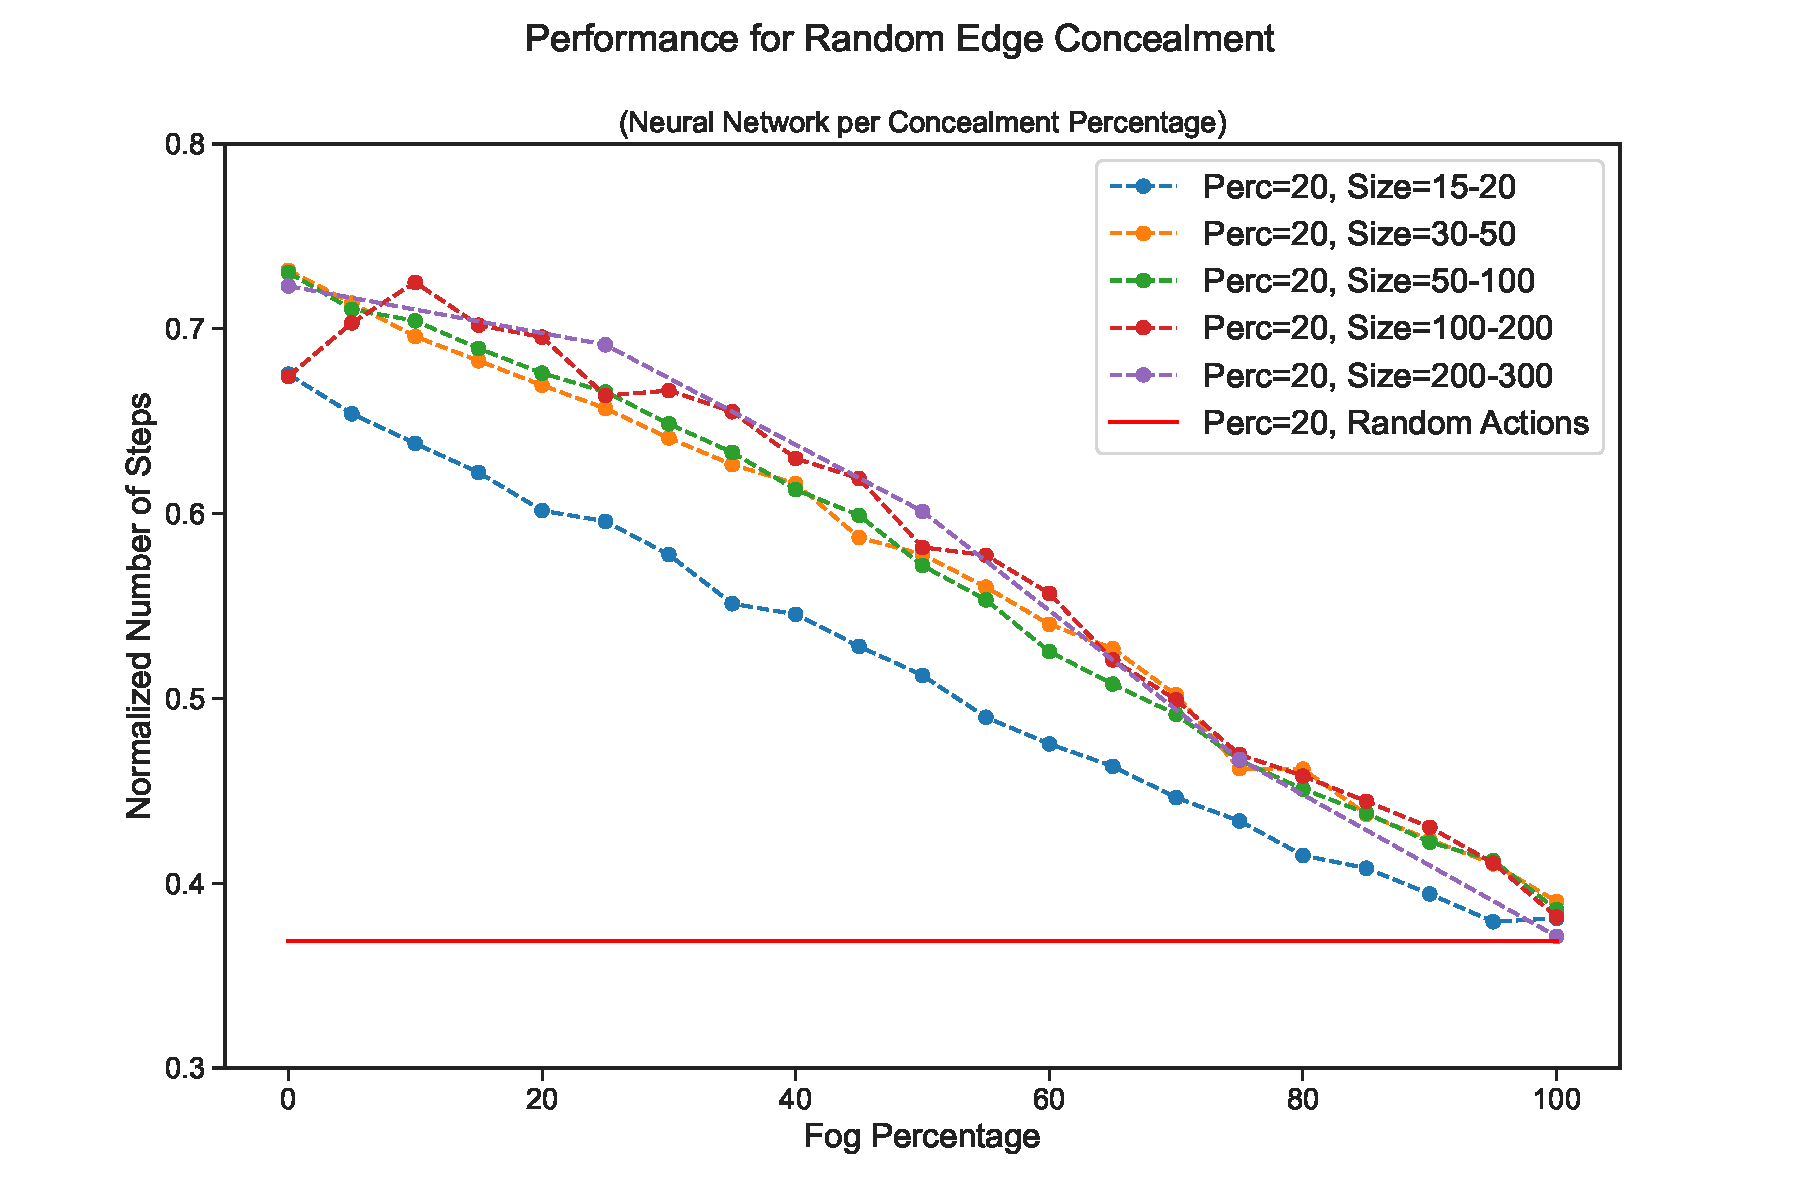
\includegraphics[scale=0.49]{Figures/percolation20_n200-300_k2-6_g2-3_random,all_fog.pdf}
    \caption[Caption Information]{\blindtext}
    \label{figure:random uniform (all models)}
\end{figure}

\begin{figure}[ht]
\sffamily\bfseries
    \centering
    % \textbf{Random Edge Concealment with Many Models}\par\medskip
    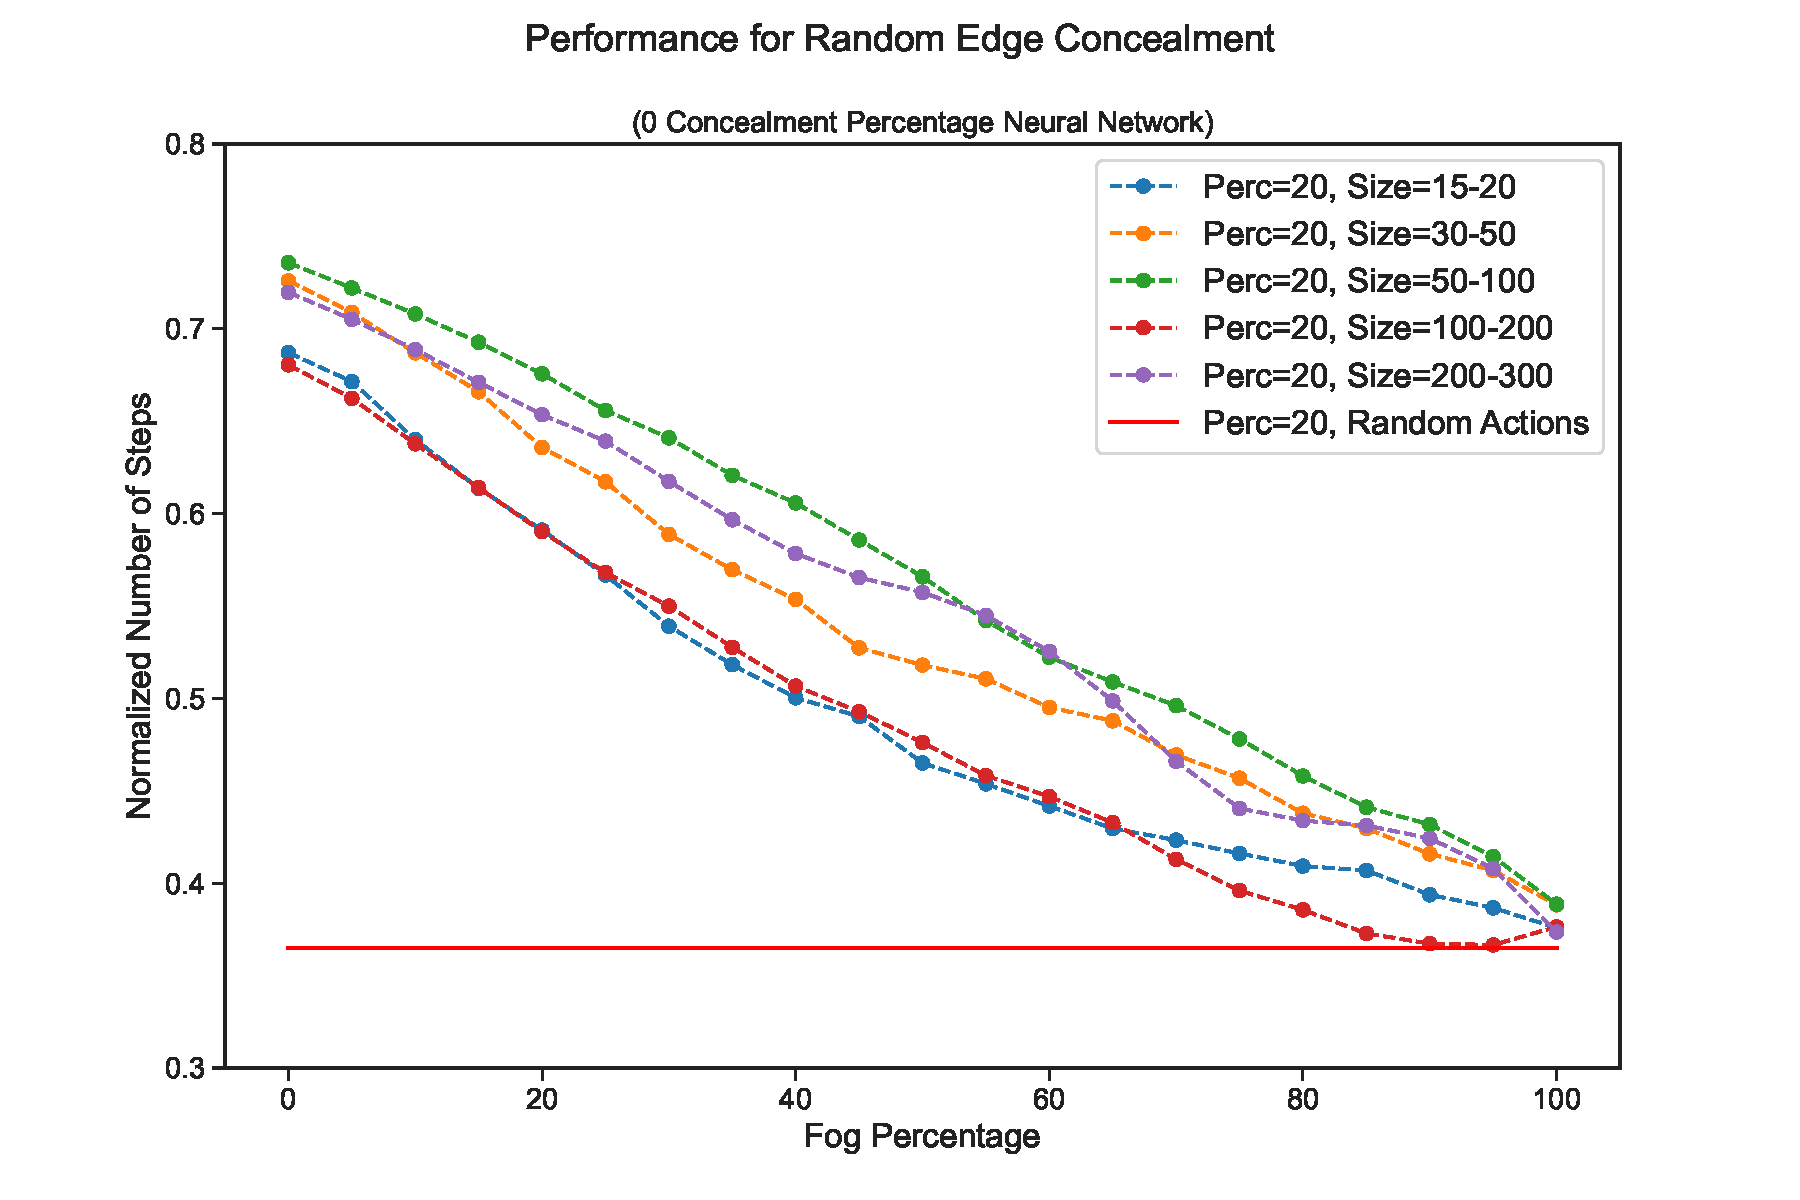
\includegraphics[scale=0.49]{Figures/percolation20_n200-300_k2-6_g2-3_p0.0_random,constant_fog.pdf}
    \caption[Caption Information]{\blindtext}
    \label{figure:random uniform (0 model)}
\end{figure}

\FloatBarrier
\clearpage
\subsection{Tabulated Performances}
% Random Edge Concealment
\begin{table}[ht]
    \centering \footnotesize
    \begin{tabular}{||c | c c ||} 
        \hline
        Network Size & \hyperref[figure:random uniform (all models)]{Area (All Models)} & \hyperref[figure:random uniform (0 model)]{Area (0.0 Model)}\\ [0.5ex] 
        \hline\hline
        15-20 & \gradient{0.13275} & \gradient{0.12930} \\ 
        \hline
        30-50 & \gradient{0.18738} & \gradient{0.17184} \\
        \hline
        50-100 & \gradient{0.18663} & \gradient{0.20129} \\
        \hline
        100-200 & \gradient{0.20822} & \gradient{0.12452} \\
        \hline
        200-300 & \gradient{0.20805}$\ast$ & \gradient{0.18448} \\ [1ex] 
        \hline
    \end{tabular}
    \caption[Caption information]{\blindtext}
    \label{table:uniform random}
\end{table}

% Discussion and Conclusion
\clearpage
% \addcontentsline{toc}{section}{Discussion}
\section{Discussion and Conclusion}
\vspace{-3em}
\subsection{Discussion}
\vspace{-2em}
\hspace{\parindent} \blindtext

\newpage
\vspace{-2em}
\subsection{Conclusion}
\vspace{-2em}
\hspace{\parindent} \blindtext


% References
\newpage
\addcontentsline{toc}{section}{References}
% \section{References}
% \vspace{-4em}
\printbibliography
% \bibliography{references.bib}
% \bibliographystyle{naturemag}
% \nocite{*}

\end{document}